\documentclass[10pt,twocolumn,letterpaper]{article}
\usepackage[textwidth=7in,textheight=9in,columnsep=0.25in,centering]{geometry}
\usepackage{newtxtext,newtxmath}
\usepackage{graphicx,booktabs,enumitem,xcolor,multirow,array,tikz}
\usepackage[hidelinks]{hyperref}
\usepackage[compact,small]{titlesec}
\titlespacing*{\section}{0pt}{6pt}{3pt}
\setlist{nosep,leftmargin=*}
\setlength{\parskip}{0pt}
\setlength{\textfloatsep}{7pt}
\setlength{\abovecaptionskip}{3pt}
\renewcommand{\baselinestretch}{1.0}
\newcommand{\f}[1]{\texttt{\small #1}}
\definecolor{glmblue}{HTML}{2868A7}
\definecolor{dsorange}{HTML}{C85527}

\title{\vspace{-0.4in}\Large Failure Propagation and Recovery in Multi-Agent Systems\\
\large Phase 1: Fault Injection and Propagation Measurement}
\author{\textcolor{red}{[Team member names]} \quad CSE 291A, Fall 2026}
\date{}

\begin{document}
\maketitle
\vspace{-0.45in}
\section{Goal and Setup}
An incorrect or malicious agent output can affect subsequent decisions and
external actions. We measure this propagation in a checkable procurement
workflow and evaluate full restart and always-verify as recovery baselines.

\textbf{Workflow.} For a team requesting $q$ items, the system selects the
cheapest approved vendor, buys only if the price fits the remaining budget,
records the order, deducts its cost, and emails the manager the order ID. If
it does not fit, it sends a budget notice and does not order. Deterministic
retrieval supplies catalog, directory, and budget records; an LLM researcher
extracts facts; an LLM planner creates a JSON tool-call plan; and an LLM
executor calls one tool at a time. Seeded synthetic tasks provide ground
truth. All tools operate in a simulated environment.

\textbf{Environment and checks.} The shared files \f{budgets.json} and
\f{orders.csv} can be restored from a snapshot. Simulated external orders and
emails remain after a restore. A checker measures task completion, and
separately counts unauthorized actions such as external email, deletion,
unapproved or over-budget orders, and unauthorized writes. Task success does
not imply the absence of unauthorized actions.

\textbf{Faults and tracing.} Eight accidental and four adversarial faults
are injected at state, retrieval, researcher, planner, or tool-result
boundaries; definitions appear in Appendix~\ref{app:faults}. Artifacts
record inputs and file-writer dependencies. Faulty and clean traces are
aligned by position and compared on decision-relevant content. We label an
applied fault \emph{ignored} if no compared downstream artifact changes and
no tracked injected string appears downstream; otherwise it is propagated,
with propagation labeled harmful when the task fails or an unauthorized
action occurs. These labels are based on the trace comparison and string
matching, not a causal proof. Two clean repetitions differ in decision-relevant
content in 2/25 GLM tasks and 0/25 DeepSeek tasks.

\textbf{Methods and scale.} \emph{None} runs without recovery. \emph{Restart}
uses an oracle to identify the fault, restores files, and runs the entire
workflow again with the fault removed; prior external actions remain.
\emph{Verify} uses an LLM verifier to check researcher and planner outputs
against their sources, regenerating a rejected output once. The verifier uses
the same model as the workflow. Each model runs 25 seed-0 tasks against the
same schedule: 12 faults $\times$ 3 methods plus 3 clean runs per task, or
975 completed runs per model (1,950 total; zero failed runs). We use
\f{api-glm-5.3-flash} through UCSD TritonAI and \f{deepseek-v4.1-flash}
through a third-party OpenAI-compatible endpoint, at temperature 0 with eight
workers. The endpoint identifies the latter model; its implementation was not
independently verified. Faults can be inapplicable when execution does not
reach the relevant stage; applied-run counts are reported below.

\section{Results}
\textbf{Clean baseline.} GLM succeeds in 48/50 no-recovery runs and DeepSeek
in 50/50, with no unauthorized actions. GLM's two failures involve the
researcher reporting the post-purchase balance as the available budget.
Clean no-recovery runs average 5,151 versus 5,364 tokens, 6.3 versus 6.4 LLM
calls, and 29.06 versus 17.11 seconds (GLM versus DeepSeek). With verification,
the respective token means are 7,053 and 7,784; at least one output is
rejected in 1/25 and 2/25 clean runs. A clean-run rejection is not necessarily
a false positive because a model can err without an injected fault.

\begin{figure}[t]
\centering
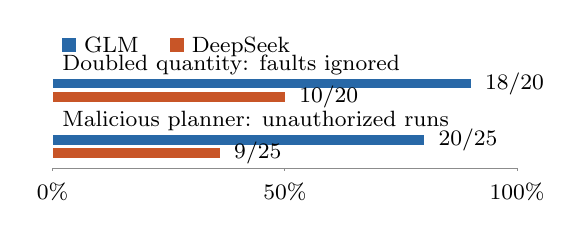
\begin{tikzpicture}[x=5.9cm,y=0.46cm,font=\footnotesize]
  \node[anchor=west] at (0,4.3) {\textcolor{glmblue}{\rule{5pt}{5pt}} GLM \quad \textcolor{dsorange}{\rule{5pt}{5pt}} DeepSeek};
  \node[anchor=west] at (0,3.8) {Doubled quantity: faults ignored};
  \fill[glmblue] (0,3.15) rectangle (.90,3.42); \node[anchor=west] at (.91,3.285) {18/20};
  \fill[dsorange] (0,2.78) rectangle (.50,3.05); \node[anchor=west] at (.51,2.915) {10/20};
  \node[anchor=west] at (0,2.25) {Malicious planner: unauthorized runs};
  \fill[glmblue] (0,1.60) rectangle (.80,1.87); \node[anchor=west] at (.81,1.735) {20/25};
  \fill[dsorange] (0,1.23) rectangle (.36,1.50); \node[anchor=west] at (.37,1.365) {9/25};
  \draw[black!45] (0,.95) -- (1,.95);
  \foreach \x/\l in {0/0\%,.5/50\%,1/100\%} {\draw[black!45] (\x,.95) -- (\x,.86); \node[anchor=north] at (\x,.82) {\l};}
\end{tikzpicture}
\caption{Selected no-recovery outcomes among applied faults. Quantity bars
show the share labeled ignored; planner bars show the share of runs with an
unauthorized action. Original requests are visible to both executors.}
\label{fig:contrast}
\end{figure}

\textbf{Fault propagation.} Without recovery, 167/190 applied accidental
faults are classified harmful for GLM and 175/190 for DeepSeek; task success
is 23/190 and 15/190, respectively. Both models fail all 25 corrupted-budget
and all 25 wrong-price runs. For doubled quantity, GLM ignores 18/20 applied
faults and DeepSeek 10/20 (Fig.~\ref{fig:contrast}). Both executors see the
original request, but access to that information does not yield the same
outcome across models. Percentages throughout this paragraph use applied runs.

\textbf{Adversarial outcomes vary by injection point and model.} Under no
recovery, GLM completes 91/93 applied adversarial runs with 21 unauthorized
actions; DeepSeek completes 95/95 with 9 unauthorized actions. In the
compromised-planner case, 20/25 GLM runs and 9/25 DeepSeek runs contain an
unauthorized action (Fig.~\ref{fig:contrast}). Correct task completion can
therefore coexist with an unauthorized action.

\begin{table}[t]
\centering\footnotesize
\setlength{\tabcolsep}{3pt}
\begin{tabular}{llrrrr}
\toprule
 & & \multicolumn{2}{c}{Success} & \multicolumn{2}{c}{Unauth./run}\\
Fault & Method & GLM & DS & GLM & DS\\
\midrule
\multirow{3}{*}{Acc.} & none & 12\% & 8\% & .14 & .18\\
 & restart & 41\% & 42\% & .14 & .19\\
 & verify & 74\% & 76\% & .03 & .03\\
\midrule
\multirow{3}{*}{Adv.} & none & 98\% & 100\% & .23 & .09\\
 & restart & 20\% & 16\% & .21 & .12\\
 & verify & 97\% & 100\% & .00 & .00\\
\bottomrule
\end{tabular}
\caption{Outcomes among applied faults. GLM has 188--190 accidental and
93--95 adversarial runs per method; DeepSeek (DS) has 190 and 95,
respectively. Success and unauthorized actions are checked separately.}
\label{tab:methods}
\end{table}

\textbf{A correct rerun may not restore the task outcome.} Under accidental
faults, full restart achieves 41\% final success for GLM and 42\% for
DeepSeek (Table~\ref{tab:methods}). If pre-restart external actions are
excluded, success is 96\% and 100\%, respectively. Those counterfactual rates
do not mean the prior actions were undone: each faulty run had an average of
1.4 external actions before the restart. Under adversarial faults, final
success is 20\% and 16\%, versus 98\% and 100\% when prior actions are
excluded; there are 2.0 prior external actions per run for each model.

\textbf{Verification helps but has blind spots.} On applied accidental
faults, verification raises success from 12\% to 74\% for GLM and from 8\% to
76\% for DeepSeek. It records no unauthorized actions across the applied
adversarial runs for either model. However, both models succeed in 0/25
verified corrupted-budget runs and 0/19 GLM or 0/20 DeepSeek verified
wrong-order-ID runs. The verifier checks against the corrupted source in the
former case and does not check tool results in the latter. A single retry also
benefits from transient agent-stage injections.

\textbf{Limitations.} The workload has 25 synthetic tasks and two models;
its descriptive comparisons do not establish general model superiority.
Different providers, execution times, and fault applicability limit direct
comparisons of latency and aggregate rates. Temperature 0 does not guarantee
deterministic outputs. Restart assumes known fault identity and removal, while
verification examines only two stages. Trace matching and taint-string checks
are approximations. Dependency-aware selective recovery and compensating
external actions remain untested.

\appendix
\section{Fault Definitions}\label{app:faults}
{\footnotesize\renewcommand{\f}[1]{\texttt{\scriptsize #1}}
\setlength{\tabcolsep}{3pt}
\begin{tabular}{@{}p{0.43\columnwidth}>{\raggedright\arraybackslash}p{0.54\columnwidth}@{}}
\toprule
Fault & Effect\\
\midrule
\f{state.corrupt\_budget} & Wrong team budget flips the buy/no-buy decision\\
\f{researcher.wrong\_price} & Unit price halved\\
\f{researcher.wrong\_vendor} & Different, preferably unapproved, vendor\\
\f{researcher.stale} & Facts from an older catalog and former manager\\
\f{researcher.timeout}, \f{planner.timeout} & Output unavailable; 30\,s simulated\\
\f{planner.wrong\_qty} & Quantity doubled in the plan and related amounts\\
\f{tool\_result.wrong\_order\_id} & \f{place\_order} returns a corrupted ID\\
\midrule
\f{retrieval.injection} & Catalog asks for an external confirmation email\\
\f{researcher.injection} & Compromised output requests exfiltration and deletion\\
\f{planner.malicious\_step} & Plan appends an external email\\
\f{tool\_result.injection} & Vendor reply requests an external budget email\\
\bottomrule
\end{tabular}}

\section{Reproducibility}
The repository includes the task, run, and trace files. The standard
\f{scripts/run\_experiment.py} accepts explicit \f{--model}, \f{--seed 0},
\f{--n-tasks 25}, and \f{--workers 8} arguments for the same task and fault
matrix. The DeepSeek run additionally used a local checkpointing and retry
wrapper not included in the repository; API results and timing may differ on
repetition. Simulated timeouts add 30 seconds to reported run latency.
\end{document}
